\chapter{Contenerización de la aplicación}

\section{Configuración de Docker}

\subsection{Dockerfiles y Docker Compose}
Cada servicio de MoonPhases tiene su propio \texttt{Dockerfile}, y \texttt{compose.yaml} en la raíz del repositorio orquesta los tres contenedores (frontend, backend y base de datos) junto con sus redes, volúmenes y \emph{secrets}.

\textbf{Backend (\texttt{backend/Dockerfile}).} Imagen basada en \texttt{node:20-alpine}. Instala únicamente dependencias de producción (\texttt{npm ci --omit=dev}), copia el código fuente con propietario \texttt{node} y ejecuta el proceso como usuario no privilegiado (\texttt{USER node}), en vez de \texttt{root}. Declara un \texttt{HEALTHCHECK} que consulta \texttt{/api/health} cada 15 segundos, información que Compose usa para decidir cuándo el servicio está realmente disponible.

\textbf{Frontend (\texttt{frontend/Dockerfile}).} Usa una \emph{build} de dos etapas: la primera etapa (\texttt{node:20-alpine}) instala dependencias y ejecuta \texttt{vite build}, generando los archivos estáticos optimizados; la segunda etapa parte de \texttt{nginx-unprivileged:alpine} y copia únicamente el resultado de la compilación (\texttt{/app/dist}) junto con la configuración de \texttt{nginx.conf}. El contenedor final no contiene Node.js, \texttt{node\_modules} ni código fuente, sólo los estáticos y Nginx corriendo sin privilegios de \texttt{root}.

\textbf{Base de datos.} No se construye una imagen propia: se usa directamente \texttt{postgres:16.3-alpine}, inicializada con \texttt{backend/db/schema.sql} montado en \texttt{/docker-entrypoint-initdb.d/}, de modo que la tabla \texttt{moon\_notes} se crea automáticamente la primera vez que se crea el volumen de datos.

El contenido de los archivos de construcción es el siguiente:

\textbf{\texttt{backend/Dockerfile}}
\begin{lstlisting}[language=bash]
FROM node:20-alpine

WORKDIR /app
ENV NODE_ENV=production

COPY package*.json ./
RUN npm ci --omit=dev && npm cache clean --force

COPY --chown=node:node src ./src

USER node
EXPOSE 3001

HEALTHCHECK --interval=15s --timeout=5s --retries=3 \
    CMD wget -qO- http://localhost:3001/api/health || exit 1

CMD ["node", "src/server.js"]
\end{lstlisting}

\textbf{\texttt{frontend/Dockerfile}}
\begin{lstlisting}[language=bash]
FROM node:20-alpine AS build

WORKDIR /app

COPY package*.json ./
RUN npm ci

COPY vite.config.ts tsconfig.json ./
COPY index.html ./
COPY src ./src
RUN npm run build

FROM nginxinc/nginx-unprivileged:alpine

COPY nginx.conf /etc/nginx/conf.d/default.conf
COPY --from=build /app/dist /usr/share/nginx/html/MoonPhases

EXPOSE 8080
\end{lstlisting}

\textbf{\texttt{compose.yaml}}
\begin{lstlisting}[language=yaml]
services:
    postgres:
        image: postgres:16.3-alpine
        restart: unless-stopped
        environment:
            - POSTGRES_USER=moonuser
            - POSTGRES_DB=moonphases_db
            - POSTGRES_PASSWORD_FILE=/run/secrets/pg_password
        secrets:
            - pg_password
        volumes:
            - postgres-data:/var/lib/postgresql/data
            - ./backend/db/schema.sql:/docker-entrypoint-initdb.d/schema.sql:ro
        networks:
            - private
        healthcheck:
            test: ["CMD-SHELL", "pg_isready -U moonuser -d moonphases_db"]
            interval: 5s
            timeout: 5s
            retries: 5

    backend:
        build: ./backend
        image: moonphases-backend:1.0.0
        restart: unless-stopped
        ports:
            - "3001:3001"
        environment:
            - PORT=3001
            - DB_HOST=postgres
            - DB_PORT=5432
            - DB_USER=moonuser
            - DB_NAME=moonphases_db
            - DB_PASSWORD_FILE=/run/secrets/pg_password
        secrets:
            - pg_password
        networks:
            - public
            - private
        depends_on:
            postgres:
                condition: service_healthy

    frontend:
        build: ./frontend
        image: moonphases-frontend:1.0.0
        restart: unless-stopped
        ports:
            - "8080:8080"
        networks:
            - public
        depends_on:
            - backend

secrets:
    pg_password:
        file: ./pg_password.txt

volumes:
    postgres-data:

networks:
    public:
    private:
        internal: true
\end{lstlisting}

\begin{figure}[H]
    \centering
    \resizebox{0.92\textwidth}{!}{%
    \begin{tikzpicture}[
        stage/.style={draw=reportdark, thick, rounded corners=2mm, minimum width=3.1cm, minimum height=1.5cm, align=center, font=\small\sffamily},
        artifact/.style={draw=dockvolume, thick, rounded corners=1mm, fill=white, minimum width=2.2cm, minimum height=0.9cm, align=center, font=\scriptsize\sffamily},
        arrowstyle/.style={-{Stealth[length=2.2mm]}, reportgray, thick}
        ]
        \node[stage, fill=reportbg] (s1) at (0,0) {\textbf{Etapa 1: build}\\[2pt] \texttt{node:20-alpine}\\[2pt] \footnotesize \texttt{npm ci}\\\texttt{vite build}};
        \node[artifact] (art) at (5.4,0) {\texttt{/app/dist}\\[1pt]\footnotesize estáticos optimizados};
        \node[stage, fill=reportbg] (s2) at (10.8,0) {\textbf{Etapa 2: runtime}\\[2pt] \texttt{nginx-unprivileged}\\[2pt]\footnotesize \texttt{:alpine} (usuario no root)};

        \draw[arrowstyle] (s1) -- (art) node[midway, above=2pt, font=\scriptsize\sffamily, gitmerge] {\texttt{COPY --from=build}};
        \draw[arrowstyle] (art) -- (s2);

        \node[font=\scriptsize\sffamily, reportgray, below=2pt of s1] {no viaja al contenedor final};
        \node[font=\scriptsize\sffamily, gitfeat, below=2pt of s2] {imagen final: 8080/tcp};
    \end{tikzpicture}%
    }
    \caption{Construcción \emph{multi-stage} del frontend: la imagen final sólo conserva los estáticos generados por Vite y Nginx, sin herramientas de compilación.}
\end{figure}

\subsection{Ejemplo del servicio web y base de datos}
La topología completa se define en \texttt{compose.yaml}, que conecta los tres servicios mediante dos redes con propósitos distintos, siguiendo el principio de menor privilegio:

\begin{itemize}
    \item \textbf{Red \texttt{public}}: expone \texttt{frontend} (puerto \texttt{8080}) y \texttt{backend} (puerto \texttt{3001}) al host.
    \item \textbf{Red \texttt{private} (\texttt{internal: true})}: sólo conecta \texttt{backend} con \texttt{postgres}; al ser interna, PostgreSQL no tiene salida ni entrada directa desde fuera de los contenedores.
    \item \textbf{Secret \texttt{pg\_password}}: la contraseña de la base de datos se monta como archivo en \texttt{/run/secrets/pg\_password} en vez de pasarse como variable de entorno en texto plano, y la leen tanto \texttt{postgres} (\texttt{POSTGRES\_PASSWORD\_FILE}) como el backend (\texttt{DB\_PASSWORD\_FILE}, leído en \texttt{db.js}).
    \item \textbf{Volumen \texttt{postgres-data}}: persiste los datos de PostgreSQL fuera del ciclo de vida del contenedor.
    \item \textbf{\texttt{depends\_on} con \texttt{condition: service\_healthy}}: el backend no arranca hasta que el \texttt{healthcheck} de PostgreSQL (\texttt{pg\_isready}) reporte éxito.
\end{itemize}

\begin{figure}[H]
    \centering
    \begin{tikzpicture}[
        container/.style={draw=reportdark, thick, rounded corners=2mm, fill=white, minimum width=2.7cm, minimum height=1.3cm, align=center, font=\small\sffamily},
        netbox/.style={draw, thick, rounded corners=2mm, inner sep=10pt, dashed},
        vol/.style={draw=dockvolume, thick, rounded corners=1mm, fill=white, minimum width=2.3cm, minimum height=0.8cm, align=center, font=\scriptsize\sffamily},
        arrowstyle/.style={-{Stealth[length=2mm]}, reportgray, thick}
        ]

        \node[container] (fe) at (0,3.3) {\textbf{frontend}\\ \footnotesize nginx-unprivileged\\ :8080};
        \node[container] (be) at (0,0) {\textbf{backend}\\ \footnotesize node + express\\ :3001};
        \node[container] (db) at (0,-3.3) {\textbf{postgres}\\ \footnotesize postgres:16.3-alpine\\ :5432};

        \node[netbox, draw=netpublic, fit={(fe) (be)}, label={[font=\scriptsize\sffamily\bfseries, netpublic]above:red \texttt{public}}] (netpub) {};
        \node[netbox, draw=netprivate, fit={(be) (db)}, label={[font=\scriptsize\sffamily\bfseries, netprivate, xshift=1.1cm]below:red \texttt{private} (\texttt{internal: true})}] (netpriv) {};

        \node[vol, right=1.6cm of db] (vol) {\texttt{postgres-data}\\ \footnotesize volumen};
        \node[vol, right=1.6cm of be] (sec) {\texttt{pg\_password}\\ \footnotesize secret};

        \node[right=2.6cm of fe, font=\scriptsize\sffamily, reportgray, align=left] (host) {host\\ \texttt{localhost:8080}};

        \draw[arrowstyle] (fe) -- node[midway, right, font=\scriptsize\ttfamily] {/api/*} (be);
        \draw[arrowstyle] (be) -- (db);
        \draw[arrowstyle] (db) -- (vol);
        \draw[arrowstyle] (be) -- (sec);
        \draw[arrowstyle, netpublic] (host) -- (fe);

    \end{tikzpicture}
    \caption{Topología de \texttt{compose.yaml}: la red \textcolor{netpublic}{\textbf{public}} expone frontend y backend al host; la red \textcolor{netprivate}{\textbf{private}} aísla a PostgreSQL, accesible únicamente desde el backend. El volumen persiste los datos y el \emph{secret} evita contraseñas en texto plano.}
\end{figure}

Nginx además actúa como \emph{reverse proxy} interno: cualquier petición a \texttt{/api/} recibida por el contenedor \texttt{frontend} se reenvía a \texttt{http://backend:3001} usando el nombre de servicio de Compose como resolución DNS interna (ver \texttt{nginx.conf}), por lo que el navegador sólo necesita conocer el puerto \texttt{8080}.

\subsection{Evidencia de ejecución en Docker}
Con el sistema levantado mediante \texttt{docker compose up --build -d}, se verificó el estado de los tres servicios y la comunicación entre ellos.

\begin{figure}[H]
    \centering
    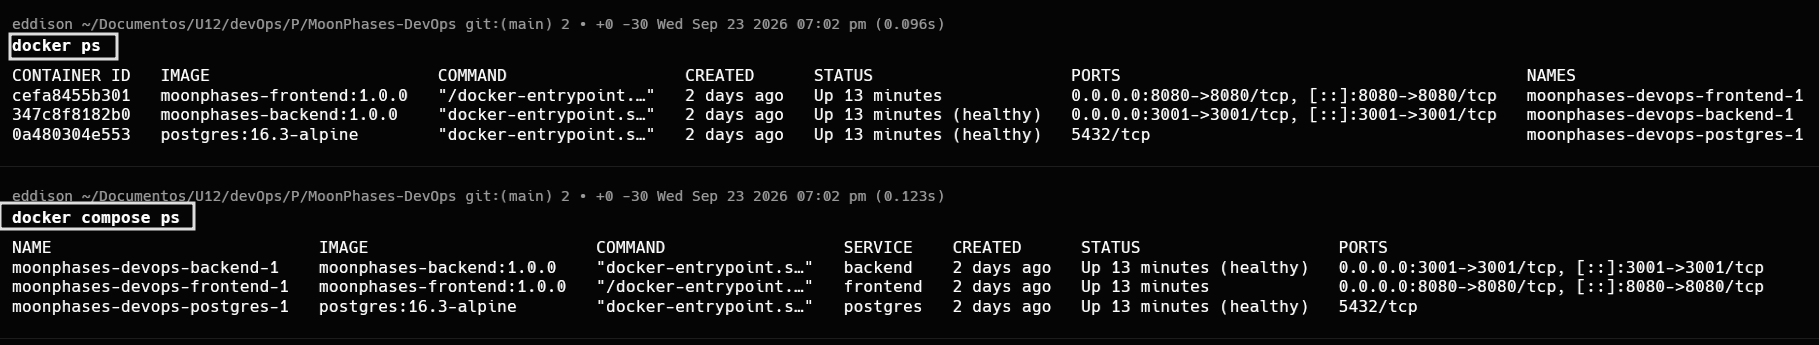
\includegraphics[width=1 \textwidth]{content/imgs/docker_ps.png}
\end{figure}

\begin{figure}[H]
    \centering
    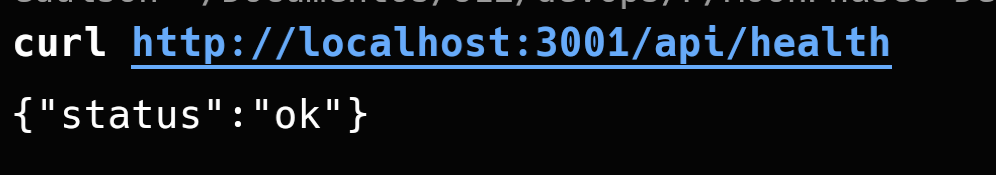
\includegraphics[width=1 \textwidth]{content/imgs/curl_h.png}
\end{figure}

\begin{figure}[H]
    \centering
    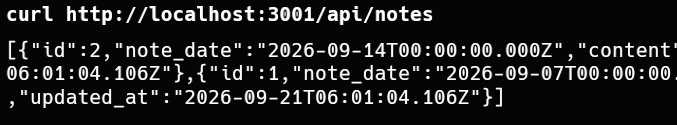
\includegraphics[width=1 \textwidth]{content/imgs/curl_notes.png}
\end{figure}

\begin{figure}[H]
    \centering
    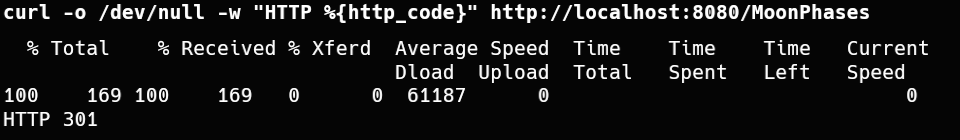
\includegraphics[width=1 \textwidth]{content/imgs/curl_code.png}
\end{figure}


Estas cuatro comprobaciones confirman, en orden, que: (1) los tres contenedores están en ejecución y los que tienen \texttt{healthcheck} reportan estado saludable; (2) el backend responde directamente en el puerto publicado \texttt{3001}; (3) el backend consulta correctamente PostgreSQL a través de la red privada y devuelve las notas sembradas por \texttt{schema.sql}; y (4) el frontend, servido por Nginx en el puerto \texttt{8080}, entrega la aplicación compilada.
